\section{The Higgs Boson}%
\label{sec:higgs_boson}

The Higgs boson is the only scalar particle in the SM. It is massive and has
neither electric nor colour charge. The Higgs boson couples to all massive
particles, including itself, with coupling strengths monotonically related to
the particle's mass. In particular, the coupling to gauge bosons, $V$, and
fermions is proportional to $m_V^2$ and $m_f$, respectively.
% The coupling of the Higgs boson to gauge bosons, $V$, is proportional
% to $m_{V}^2$. Similarly, the Yukawa interactions between Higgs bosons and
% fermions are predicted to have strengths proportional to the mass of the
% fermion, $m_f$.
The detection of the Higgs boson and confirmation of its
properties (e.g.\ spin, intrinsic parity, mass-dependent coupling strengths)
would validate our current understanding of the BEH mechanism and the
Glashow--Salam--Weinberg model of the electroweak interaction.

In 2012, almost half a century after the proposal of the
Glashow--Salam--Weinberg model, the Higgs boson was discovered by the
ATLAS~\cite{HIGG-2012-27} and CMS~\cite{CMS-HIG-12-028} collaborations at the
LHC with a mass of about \SI{125}{\GeV}. Since its discovery, extensive
measurements of its properties have been performed showing remarkable agreement
with the SM predictions. In 2022, the Higgs boson mass has been measured with a
relative error approaching \SI{0.1}{\percent}. At the time of writing, the most
precise measurement of the Higgs boson mass by the ATLAS collaboration yields
\begin{align*}
  m_{H} = \num{124.94}%
  \valuesep\numerrt{0.17}{stat.}%
  \valuesep\numerrt{0.03}{syst.}%
  \valuesep\si{\GeV}
\end{align*}
in the $H \to Z Z^{*} \to 4\ell$ channel~\cite{HIGG-2020-07} using \pp~collision
events recorded in the period from 2011--2012 and 2015--2018. The observed Higgs
boson is compatible with the scalar particle
hypothesis~\cite{HIGG-2013-17-witherratum,CMS-HIG-14-018} and its coupling
strengths are in good agreement with the SM
predictions~\cite{HIGG-2021-23,CMS-HIG-22-001}. The EWSB in the SM is now
well-established and its free parameters, $\varv$ and $m_{H}$, determined with
high precision.\footnote{The VEV was known prior to the discovery of the Higgs
  boson through measurements of the muon lifetime, which determines the
  effective coupling constant $G_{\text{F}}$ of the charged-current weak
  interaction. With known $G_{\text{F}}$, the VEV can be calculated according to
  $\varv = \bigl( \sqrt{2} G_{\text{F}} \bigr)^{-1/2} \approx
  \SI{246}{\GeV}$~\cite{MuLan:2010shf}.}


\subsection{Production and Decay Modes}

The production of Higgs bosons at the LHC occurs through different production
modes. Feynman diagrams of the four dominant ones are shown in
\Cref{fig:higgs_prod_feyn}, all of which have been experimentally confirmed to
exist. The Higgs boson production cross section in \pp~collisions at a
centre-of-mass energy of \SI{13}{\TeV} is shown in \Cref{fig:higgs_prod_xsec} as
a function of $m_{H}$. For $m_{H} = \SI{125.0}{\GeV}$, the gluon--gluon fusion
(\ggF) production mode has the largest cross section with
$\sigma(\pp \to H) \approx \SI{50}{\pico\barn}$, followed by the vector
boson fusion (VBF) mode with $\sigma(\pp \to qqH) \approx \SI{4}{\pico\barn}$,
the $VH$ mode with $\sigma(\pp \to VH) \approx \SI{2}{\pico\barn}$ for
$V = W^\pm$ or $Z$, and finally the $\ttbar H$ mode with
$\sigma(\pp \to \ttbar H) \approx
\SI{0.5}{\pico\barn}$~\cite{deFlorian:2016spz}.
% Higgs boson production modes involving two Higgs bosons in the final state,
% which are the processes of primary interest for this thesis, are covered in
% \Cref{fig:theory_higgs_pair_prod}.

\begin{figure}[htbp]
  \centering

  \begin{subfigure}{0.48\textwidth}
    \centering
    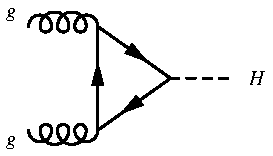
\includegraphics[scale=1]{feynman_graphs/higgs_prod_ggf}
    \subcaption{Gluon--gluon fusion (\ggF)}
  \end{subfigure}%
  \begin{subfigure}{0.48\textwidth}
    \centering
    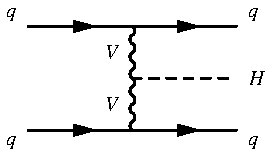
\includegraphics[scale=1]{feynman_graphs/higgs_prod_vbf}
    \subcaption{Vector boson fusion (VBF)}
  \end{subfigure}

  \vspace*{0.5em}

  \begin{subfigure}{0.48\textwidth}
    \centering
    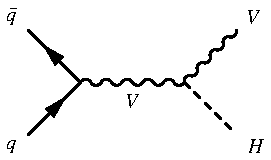
\includegraphics[scale=1]{feynman_graphs/higgs_prod_vh}
    \subcaption{Associated production with a massive vector boson ($VH$)}
  \end{subfigure}%
  \begin{subfigure}{0.48\textwidth}
    \centering
    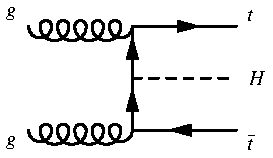
\includegraphics[scale=1]{feynman_graphs/higgs_prod_tth}
    \subcaption{Associated production with \ttbar ($\ttbar H$)}
  \end{subfigure}%

  \caption[Higgs boson production modes in \pp~collisions.]{The dominant Higgs
    boson production modes in \pp~collisions at centre-of-mass energies of
    \SI{13}{\TeV}.}%
  \label{fig:higgs_prod_feyn}
\end{figure}

\begin{figure}[htbp]
  \centering

  \begin{subfigure}[b]{0.47\textwidth}
    \centering

    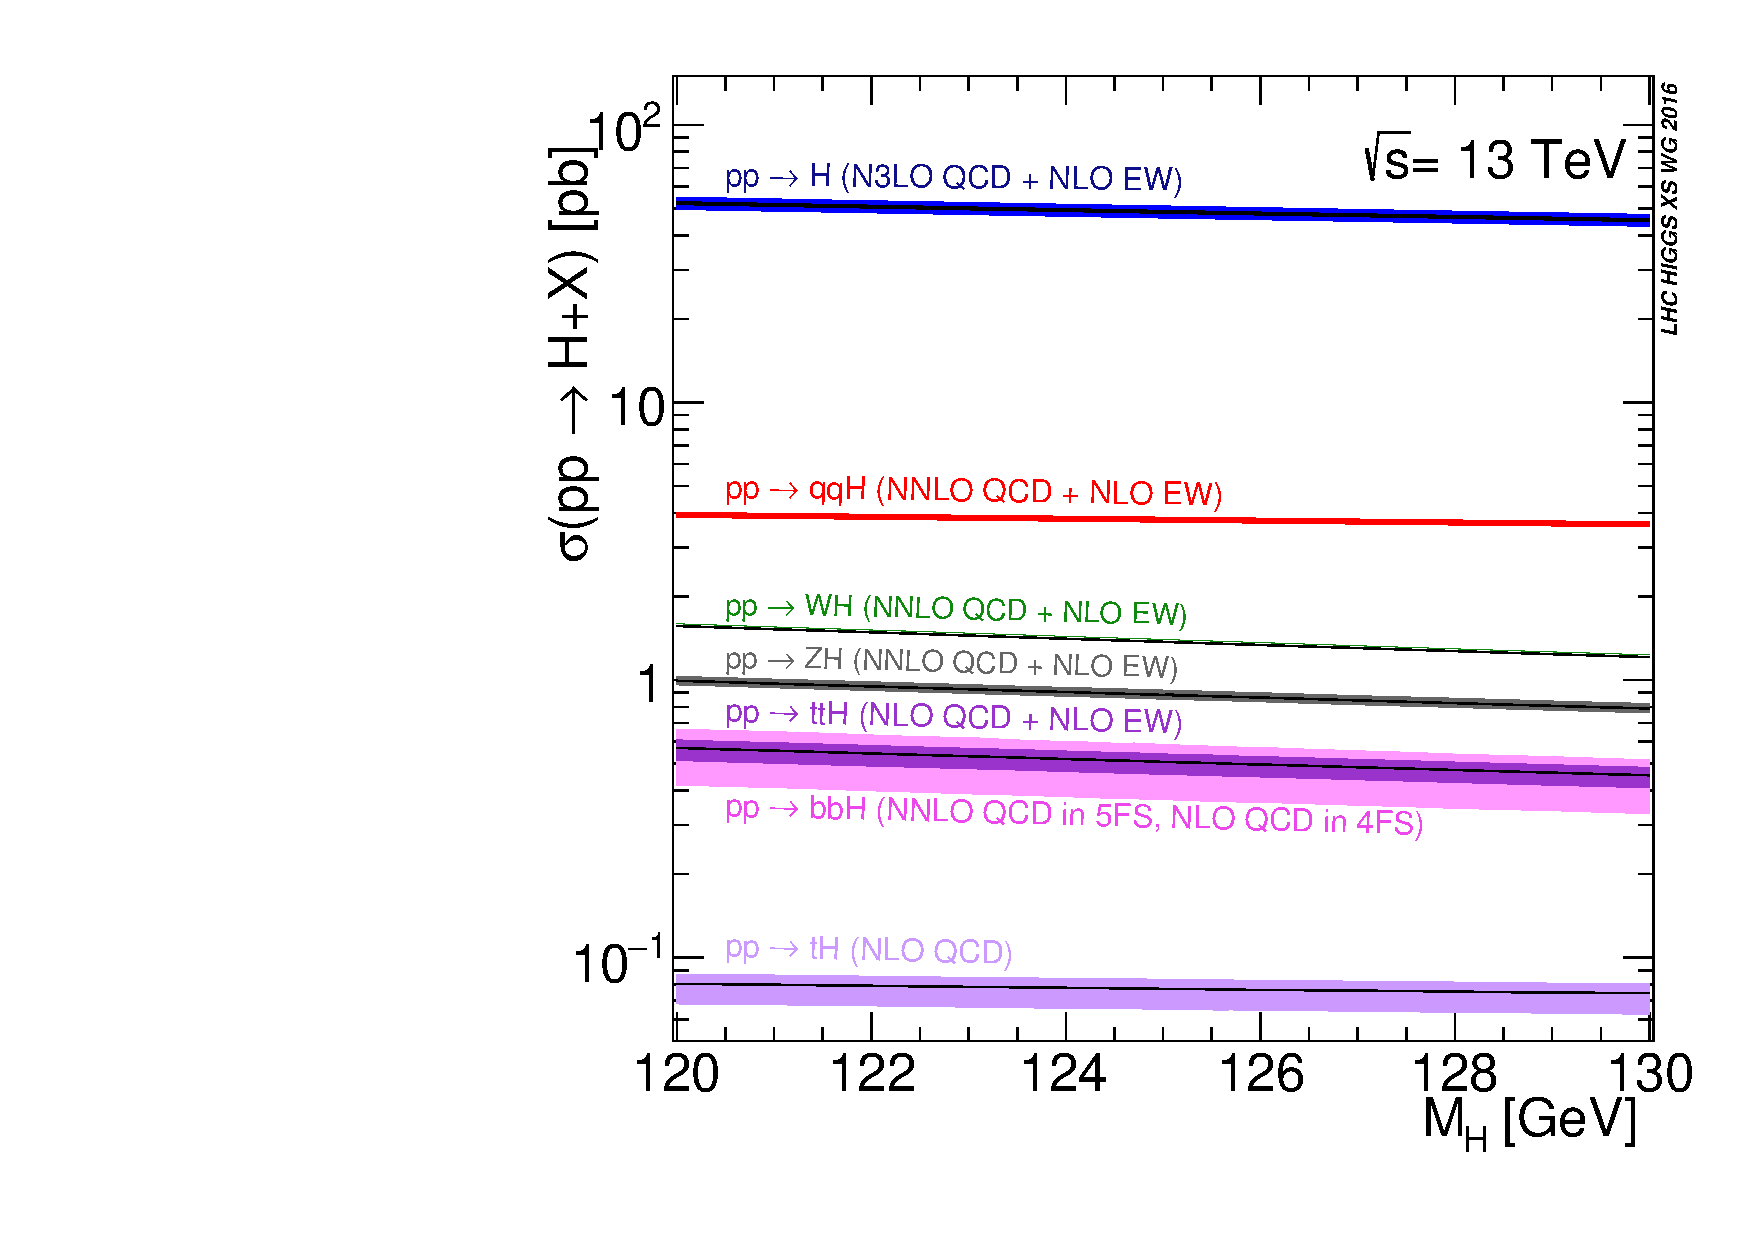
\includegraphics[width=0.95\textwidth]{theory/h_prod_crossec_13tev}

    \subcaption{Cross sections of Higgs boson production modes as a function of
      $m_{H}$.\\}%
    \label{fig:higgs_prod_xsec}
  \end{subfigure}\hfill%
  \begin{subfigure}[b]{0.47\textwidth}
    \centering

    {
      \renewcommand{\arraystretch}{1.1}%
      \begin{tabular}{lS[table-format=2.3]c}
  \toprule
  Decay mode  & {BR / \%} & Observed \\
  \midrule
  $\bbbar$        & 58    & \checkmark \\
  $W^{+} W^{-}$    & 21    & \checkmark \\
  $gg$            & 8.2   & \\
  $\tau^+ \tau^-$ & 6.3   & \checkmark \\
  $c\bar{c}$      & 2.9   & \\
  $ZZ^{*}$            & 2.6   & \checkmark \\
  $\gamma\gamma$  & 0.23  & \checkmark \\
  $Z\gamma$       & 0.15  & \\
  $\mu^{+}\mu^{-}$ & 0.022 & $\sim$~\cite{CMS-HIG-19-006} \\
  \bottomrule
\end{tabular}

%%% Local Variables:
%%% mode: latex
%%% TeX-master: "../phd_thesis"
%%% End:

    }

    \vspace*{1.5em}

    \subcaption{Branching ratios (BR) of the Higgs boson. The $gg$,
      $\gamma\gamma$, and $Z\gamma$ decay modes occur via higher-order
      processes. $*$:~First evidence of $H \to \mu^+ \mu^-$ decays
      exists~\cite{CMS-HIG-19-006}.}%
    \label{tab:higgs_branching_ratios}
  \end{subfigure}

  \caption[Higgs boson production cross section and branching ratios.]{Higgs
    boson production cross section in \pp~collisions at a centre-of-mass energy
    of \SI{13}{\TeV} (a) and Higgs boson branching ratios for
    $m_{H} = \SI{125.0}{\GeV}$ (b). The figure and branching ratios are taken
    from Ref.~\cite{deFlorian:2016spz}.}
\end{figure}

The Higgs boson is predicted to have a total decay width of about
\SI{4}{\MeV}~\cite{deFlorian:2016spz} yielding a proper lifetime of
$10^{-22}\,\si{\second}$. Therefore, the Higgs boson decays almost immediately
via one of the decay modes summarised in \Cref{tab:higgs_branching_ratios},
allowing detection only using its decay products. The table reflects the
preferential coupling of the Higgs boson to heavy particles such as the massive
gauge bosons\footnote{The decays of Higgs bosons to $W^+W^-$ and $ZZ$ are
  suppressed since $m_{H} < 2 m_{W} < 2 m_{Z}$ such that one of the gauge bosons
  has to be produced \emph{off-shell}.} and third generation fermions. The vast
majority of Higgs bosons decay into \bbbar with a branching ratio of
\SI{58}{\percent}. The $b$-quark is the heaviest fermion that can be produced in
the Higgs boson decay, decays to top-quark pairs being forbidden due to
$2 m_t \gg m_H$. The second most abundant fermionic Higgs boson decay mode is
$H \to \tau^+ \tau^-$ with a branching ratio of \SI{6.3}{\percent}. The
$H \to \bbbar$ and $H \to \tau^+ \tau^-$ decay modes are among the most
important probes of Yukawa interactions in the SM.
% In addition, a first indication of SM-like Yukawa couplings to fermions of the
% second generation exist in the form of evidence for the process
% $H \to \mu^+ \mu^-$ by the CMS collaboration~\cite{CMS-HIG-19-006}.


\subsection{Higgs Boson Pair Production}%
\label{fig:theory_higgs_pair_prod}

% Super excellent talk by Katharine:
% https://indico.cern.ch/event/1065153/attachments/2351166/4011032/Seminar.pdf

After the discovery of the Higgs boson and the measurement of its mass, the free
parameters of the EWSB, $\varv$ and $m_H$, are determined and thus the shape of
the BEH potential in the SM. An important test of the SM is the measurement of
processes involving the Higgs boson self-coupling. These processes can be used
to measure the cubic and quartic terms of the BEH potential directly, which is
instrumental to validate the consistency of the theory. Measurements of the
trilinear and quartic Higgs boson self-couplings can be performed in final
states with two or three Higgs bosons, respectively. The determination of the
quartic self-coupling is currently infeasible due to the small cross section of
triple Higgs boson production of about \SI{80}{\atto\barn} in \pp~collisions at
$\sqrt{s} = \SI{13}{\TeV}$~\cite{Maltoni:2014eza}. Instead, the focus of this
thesis lies in searching for Higgs boson pair production and, in doing so, probe
the trillinear Higgs boson self-coupling.\footnote{The Higgs boson self-coupling
  can also be probed indirectly through higher-order corrections to the
  production of single Higgs bosons. See for example
  Refs.~\cite{Degrassi:2016wml,ATLAS-CONF-2022-050}.}

% Mention this somewhere?
% \lambda &\approx 0.13 \quad \text{(SM)}

The production of Higgs boson pairs at the LHC is a rare process with
cross sections about 1000 times smaller than the production of single Higgs
bosons. Under the SM hypothesis, Higgs boson pair production is not yet
accessible using data collected during Run~2 of the LHC; however, first evidence
is likely to be obtained by the end of the LHC
programme~\cite{ATL-PHYS-PUB-2022-005}. Nevertheless, probing Higgs boson pair
production is valuable already. First, experimental methods can be developed and
improved that might culminate in a discovery. Second, possible deviations from
the SM can enhance the production of Higgs boson pairs to which searches might
be sensitive already.


\subsubsection{Production Modes}%

Higgs boson pair production in the SM (SM \HH production) proceeds
non-resonantly via different production modes yielding final states with two
on-shell Higgs bosons. The following description of the SM \HH production modes
assumes \pp~collisions at $\sqrt{s} = \SI{13}{\TeV}$ and
$m_{H} = \SI{125.0}{\GeV}$.

The \ggF process is the dominant SM \HH production mode. The leading order
diagrams of this process are depicted in \Cref{fig:dihiggs_ggf_feyn}. Both
diagrams involve a loop of heavy quarks, the loop being dominated by top-quarks
due to their large coupling to the Higgs boson. The box diagram depicted in
\Cref{fig:dihiggs_ggf_feyn_box} does not involve any Higgs boson
self-interaction vertices.
% \footnote{As a result, Higgs boson pair production exists even in the absence
% of Higgs boson self-interactions.}
However, the triangle diagram in
\Cref{fig:dihiggs_ggf_feyn_triangle} does involve the Higgs boson self-coupling
thus making SM $HH$ production sensitive to $\lambda_{HHH}$. The triangle and
the box diagram interfere destructively leading to a small SM $HH$ production
cross section via \ggF of
\begin{align*}
  \sigma(pp \to HH) = \SI{31.05}{\femto\barn}
  \quad \text{with} \quad
  \Delta \sigma / \sigma = \valuesep^{+\phantom{2}7\,\%}_{-23\,\%}
  % \sigma(pp \to HH) = \SIpmerr{31.1}{+2.1}{-7.2}{\femto\barn}
  %\sigma(pp \to HH) = (31.05\valuesep^{+\phantom{2}7\,\%}_{-23\,\%})\valuesep\si{\femto\barn}
\end{align*}
at NNLO~\FTapprox~\cite{Grazzini:2018bsd,Baglio:2020wgt,LHCHWGHH}.

\begin{figure}[htbp]
  \centering

  \begin{subfigure}{0.49\textwidth}
    \centering
    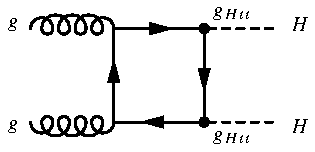
\includegraphics[width=0.7\textwidth]{feynman_graphs/di_higgs_box}
    \subcaption{}%
    \label{fig:dihiggs_ggf_feyn_box}
  \end{subfigure}\hfill%
  \begin{subfigure}{0.49\textwidth}
    \centering
    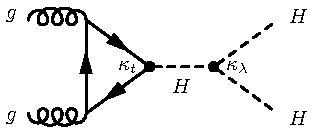
\includegraphics[width=0.7\textwidth]{feynman_graphs/di_higgs_triangle}
    \subcaption{}%
    \label{fig:dihiggs_ggf_feyn_triangle}
  \end{subfigure}

  \caption[Feynman diagrams of non-resonant Higgs boson pair production via
  \ggF.]{Feynman diagrams of non-resonant Higgs boson pair production via \ggF
    at leading order. The diagrams (a) and (b) are commonly referred to as the
    box and triangle diagrams, respectively. The Higgs boson self-coupling is
    denoted as $\lambda_{HHH}$ and the top-quark Yukawa coupling as $g_{Htt}$.}%
  \label{fig:dihiggs_ggf_feyn}
\end{figure}

The second largest SM \HH production mode is VBF, the leading order diagrams
being depicted in \Cref{fig:dihiggs_vbf_feyn}. The diagrams involve the coupling
of the Higgs boson to vector bosons, $g_{HVV}$, the quartic $HHVV$ coupling,
$g_{HHVV}$, and the Higgs boson self-coupling. A characteristic feature of the
VBF production mode is the presence of two additional jets originating from the
fragmentation and hadronisation of the final state quarks. The predicted SM \HH
production cross section via VBF is
\begin{align*}
  \sigma(\pp \to qqHH) = \SI{1.726}{\femto\barn}
  \quad \text{with} \quad
  \Delta \sigma / \sigma = \pm 2.1\,\%
\end{align*}
at $\text{N}^3\text{LO}$~\cite{Dreyer:2018qbw,LHCHWGHH}. Due to the small
cross section, the VBF production mode is currently of lesser importance to
probe the nature of the Higgs boson self-coupling.

\begin{figure}[htbp]
  \centering

  \begin{subfigure}{0.33\textwidth}
    \centering
    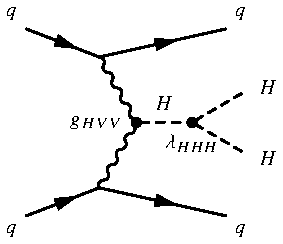
\includegraphics[width=0.95\textwidth]{feynman_graphs/di_higgs_vbf_kvklam}
    \subcaption{}
  \end{subfigure}\hfill%
  \begin{subfigure}{0.33\textwidth}
    \centering
    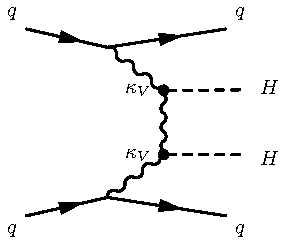
\includegraphics[width=0.95\textwidth]{feynman_graphs/di_higgs_vbf_kvkv}
    \subcaption{}
  \end{subfigure}\hfill%
  \begin{subfigure}{0.33\textwidth}
    \centering
    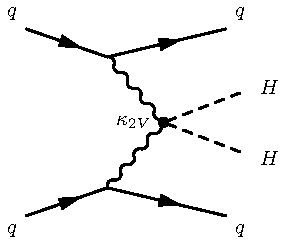
\includegraphics[width=0.95\textwidth]{feynman_graphs/di_higgs_vbf_ktwov}
    \subcaption{}
  \end{subfigure}

  \caption[Feynman diagrams of non-resonant Higgs boson pair production via
  VBF.]{Feynman diagrams of non-resonant Higgs boson pair production via VBF at
    leading order.}%
  \label{fig:dihiggs_vbf_feyn}
\end{figure}

Additional production modes of SM \HH with even smaller cross sections
exist. Examples of these are the associated production of \HH with massive
vector bosons with
$\sigma(\pp \to VHH) \approx \SI{0.9}{\femto\barn}$~\cite{deFlorian:2016spz}
($V = W^\pm$ or $Z$) and associated production with \ttbar with
$\sigma(\pp \to \ttbar HH) \approx
\SI{0.8}{\femto\barn}$~\cite{deFlorian:2016spz}. These production modes are not
considered in this thesis.


\subsubsection{Decay Channels of Pairs of SM Higgs Bosons}%

With the observed mass of the Higgs boson of about \SI{125}{\GeV}, many Higgs
boson decay modes are of interest to probe the nature of the EWSB in the
SM. When considering decays of Higgs boson pairs, this results in a plethora of
final states with often distinct signatures. An overview of the branching ratios
of a system of two SM Higgs bosons is given in \Cref{fig:hh_branching_ratios}.

\begin{figure}[htbp]
  \centering

  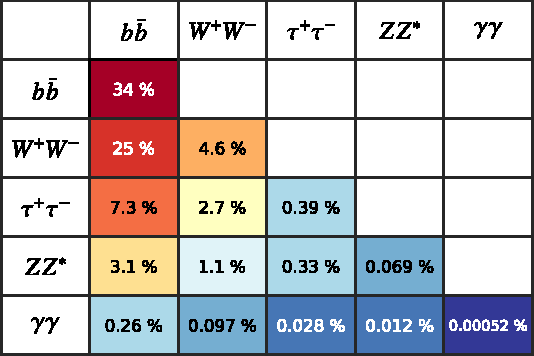
\includegraphics[width=0.5\textwidth]{theory/di_higgs_branching_ratio}

  \caption[Branching ratios of a system of two SM Higgs bosons.]{Branching
    ratios of the decay of a system of two SM Higgs bosons. The Higgs boson
    branching ratios are taken from Ref.~\cite{deFlorian:2016spz} and
    assume~$m_{H} = \SI{125.0}{\GeV}$.}%
  \label{fig:hh_branching_ratios}
\end{figure}

Experimental searches for SM \HH production have to make a compromise between
the branching ratio of the decay channel, the ability to select the relevant SM
\HH events, and the background contributions of other processes. Currently, the
search channels most sensitive to SM \HH production are:
\begin{description}

\item[The \bbbb channel] has the largest branching ratio (\SI{34}{\percent}) of
  any final state. However, this channel is dominated by backgrounds from
  multi-jet production due to its fully hadronic final state. This makes
  searches in the \bbbb channel challenging. First, the signal acceptance is
  limited due to the use of $b$-jet triggers with strict \pT~thresholds and the
  requirement of four $b$-tagged jets. Second, the reconstruction of
  $H \to \bbbar$ candidates in \bbbb final states is ambiguous, which introduces
  combinatorial backgrounds and a non-negligible fraction of misreconstructed
  signal events. Lastly, the modelling of the multi-jet background is difficult
  and introduces uncertainties that degrade the sensitivity of this channel.
  % Moreover, identifying the individual $H \to \bbbar$ candidates
  % -> Not a huge problem for SM

\item[The \bbtautau channel] has a reduced branching ratio of
  \SI{7.3}{\percent}, yet the presence of two \tauleptons provides a distinct
  signature to select signal events and to suppress the multi-jet
  background. The relevant backgrounds in this channel are the production of
  \ttbar, \Zjets, multi-jet, and single Higgs bosons events. Searches for SM \HH
  in the \bbtautau channel often focus on final states with one leptonic and one
  hadronic \taulepton decay (\lephad), and final states with two hadronic
  \taulepton decays (\hadhad). These final states cover almost \SI{90}{\percent}
  of $HH \to \bbtautau$ events.

\item[The \bbyy channel] has a very small branching ratio of
  \SI{0.26}{\percent}, but the photon pair provides an outstanding signature to
  select signal events. The di-photon invariant mass, $m_{\gamma\gamma}$, can be
  reconstructed with a mass resolution of \SIrange{1}{2}{\GeV} in the ATLAS and
  CMS detectors~\cite{PERF-2007-01,CMS-CMS-00-001}.\footnote{Compared to the
    typical resolutions of $H \to \bbbar$ and $H \to \tautau$ reconstruction in
    the \bbbb and \bbtautau channels, this represents an improvement of about an
    order of magnitude.} Therefore, $m_{\gamma\gamma}$ provides an excellent
  discriminant to reject most background processes leaving only continuum
  $\gamma\gamma$ production and single Higgs boson production as relevant
  backgrounds.

\end{description}

%%% Local Variables:
%%% mode: latex
%%% TeX-master: "../../phd_thesis"
%%% End:
